YOLO (You Only Look Once), \cite{DBLP:journals/corr/RedmonDGF15}, je inspiriran načinom na koji ljudi prepoznaju objekte. Ljudima je dovoljno da jednom pogledaju sliku i odmah znaju koji objekti se nalaze na slici i njihove lokacije što im omogućava obavljanje kompleksnih zadataka, kao što je vožnja, bez puno razmišljanja. 
Drugi detektori objekata koriste klasifikatore koje evaluiraju na različitim dijelovima slike. Neki koriste klizeći prozor pa klasifikator evaluiraju na svakoj lokaciji u slici, dok drugi koriste različite metode za predlaganje regija. YOLO detekciju objekata postavlja kao problem regresije i odjednom predviđa lokaciju i razred objekta iz piksela slike na ulazu. Model se sastoji od konvolucijske mreže s 24 konvolucijska sloja i na izlazu 2 potpuno povezana sloja. Izlazni sloj mreže koristi linearnu aktivacijsku funkciju, a ostali slojevi koriste funkciju:
\[
	\phi (x) = 
	\begin{cases}
		x, \quad \quad za \quad x > 0 \\
		0.1x, \quad inace
	\end{cases}
\]
 Arhitektura mreže prikazana je na slici \ref{yolo_mreza}. Mreža na ulazu očekuje sliku dimenzija $448 \times 448$ pa se slici prije detekcije treba promijeniti veličina ako nije zadane veličine. Slika na ulazu se dijeli na mrežu dimenzija $S \times S$. Ako sredina objekta pada u pojedinu ćeliju mreže, ta ćelija je odgovorna za detekciju tog objekta. Svaka ćelija predviđa $B$ prozora i za svaki predviđa vjerojatnost da se u tom prozoru nalazi objekt. Svaka predikcija prozora se sastoji od 5 brojeva: $x$ i $y$ koordinate središta, relativne visine i širine i vjerojatnosti da se u prozoru nalazi objekt. Budući da je svaka ćelija odgovorna za predviđanje jednog objekta, vjerojatnosti pripadnosti svakom od $C$ razreda se predviđaju jednom za svaku ćeliju, bez obzira na parametar $B$. Uz zadane parametre, izlaz YOLO mreže je tenzor dimenzija $S \times S \times (B \ast 5 + C)$. Višestruke detekcije se rješavaju tako da se prvo odbace sve detekcije čija je pouzdanost ispod zadanog praga. Nakon toga se za svaki razred uzima detekcija s maksimalnom pouzdanošću i odbacuju se sve detekcije s manjom pouzdanošću koje imaju velika preklapanja (omjer presjeka i unije veći od 0.5) s odabranom detekcijom. Postupak se ne ponavlja dok ne ostanu samo detekcije koje nemaju omjer presjeka i unije s detekcijama istog razreda veći od 0.5. Detekcija objekata YOLO modelom prikazana je na slici \ref{yolo_detekcija}. Za treniranje mreže se koristi sljedeća funkcija pogreške:
\begin{multline}
 	\lambda_{coord} \sum\limits_{i=0}^{S^2} \sum\limits_{j=0}^{B} \mathbbm{1}_{ij}^{obj}[(x_i - \hat{x}_i )^2 + (y_i - \hat{y_i})^2] \\
 	+ \lambda_{coord} \sum\limits_{i=0}^{S^2} \sum\limits_{j=0}^{B} \mathbbm{1}_{ij}^{obj} [(\sqrt{w_i} - \sqrt{\hat{w}_i})^2 + (\sqrt{h_i} - \sqrt{\hat{h}_i})^2] \\
 	+ \sum\limits_{i=0}^{S^2} \sum\limits_{j=0}^{B} \mathbbm{1}_{ij}^{obj}(C_i - \hat{C}_i)^2 \\
 	+ \lambda_{noobj} \sum\limits_{i=0}^{S^2} \sum\limits_{j=0}^{B} \mathbbm{1}_{ij}^{noobj}(C_i - \hat{C}_i)^2 \\
 	+ \sum\limits_{i=0}^{S^2} \mathbbm{1}_{i}^{obj} \sum\limits_{c \ \epsilon \ razredi} (p_i(c) - \hat{p}_i(c))^2
\end{multline}
gdje $\mathbbm{1}_{i}^{obj}$ označava nalazi li se objekt u ćeliji $i$, a $\mathbbm{1}_{ij}^{obj}$ je li $j$-ti prozor u ćeliji $i$ zadužen za predviđanje objekta. Funkcija pogreške kažnjava pogreške klasifikacije ako se objekt nalazi u ćeliji i kažnjava pogrešku u predviđenim koordinatama samo ako je prozor zadužen za predviđanje objekta. Budući da bi kažnjavanjem visine i širine direktno, jače kažnjavala pogreške kod detekcije velikih objekata, funkcija pogreške koristi korijen visine i širine za izračun pogreške. Kvadratna pogreška jednako kažnjava pogrešku klasifikacije i lokalizacije. Puno ćelija u slici ne sadrži objekt pa pouzdanost tih ćelija teži prema nuli, dok je gradijent ćelija u kojima se nalazi objekt prevelik što može uzrokovati ranu divergenciju. Taj problem se rješava tako da se poveća utjecaj pogreške predikcije koordinata prozora i smanji utjecaj pogreške klasifikacije što se postiže parametrima $\lambda_{coord}$ i $\lambda_{noobj}$. Autori postavljaju $\lambda_{coord} = 5$ i $\lambda_{noobj} = 0.5$. YOLO je u odnosu na prijašnje modele za detekciju objekata donio velika ubrzanja, ali i on ima neka ograničenja. Budući da je slika podijeljena u mrežu i svaka ćelija mreže predviđa mali broj prozora, YOLO ima problema s detekcijom malih objekata koji se pojavljuju u skupinama kao na primjer jato ptica. Također, ima poteškoća u generalizaciji u neuobičajenim okolinama i položajima objekata koji se jako razlikuju od onih viđenih u skupu podataka za trening.
 
 \begin{figure}
	\centering
	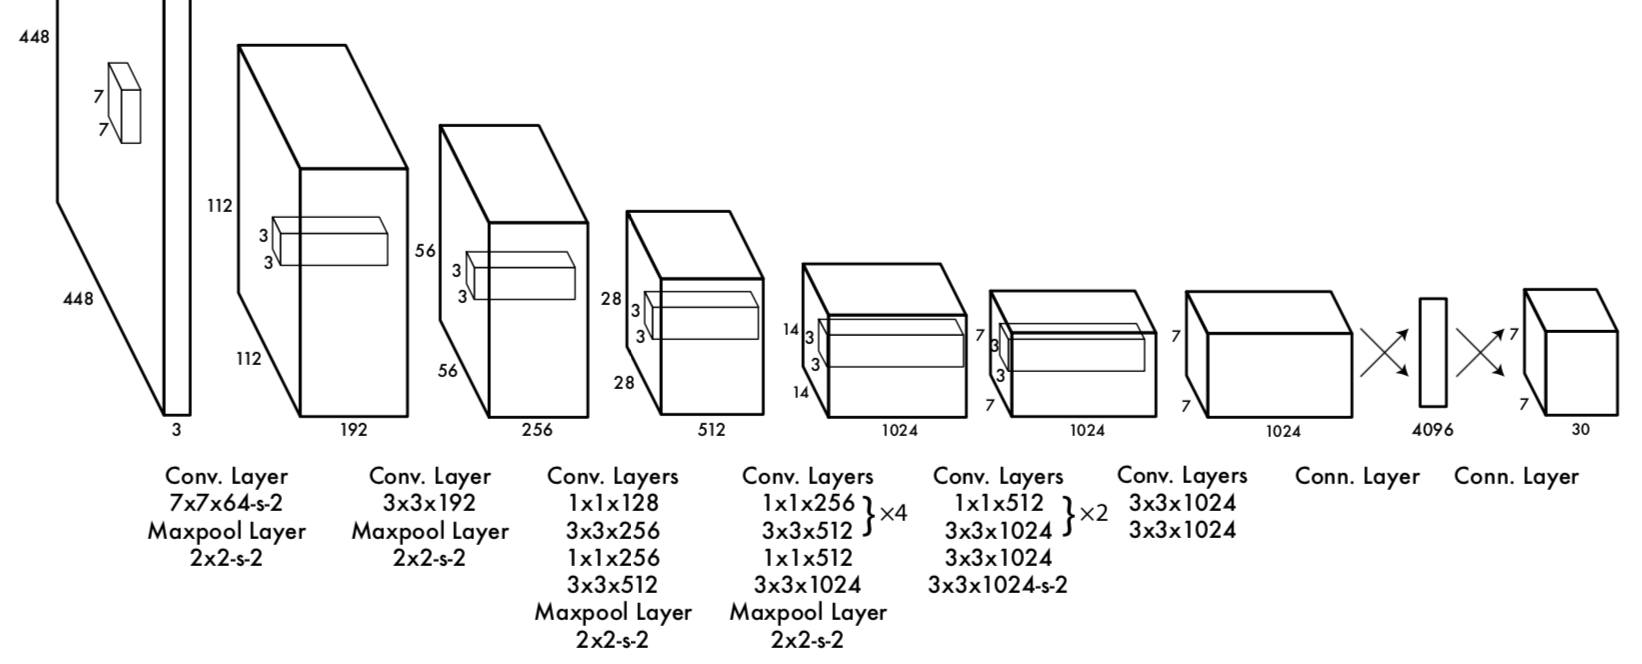
\includegraphics[scale=0.5]{img/yolo_mreza.png}
	\caption{Arhitektura YOLO mreže.}
	\label{yolo_mreza}
\end{figure}

 \begin{figure}
	\centering
	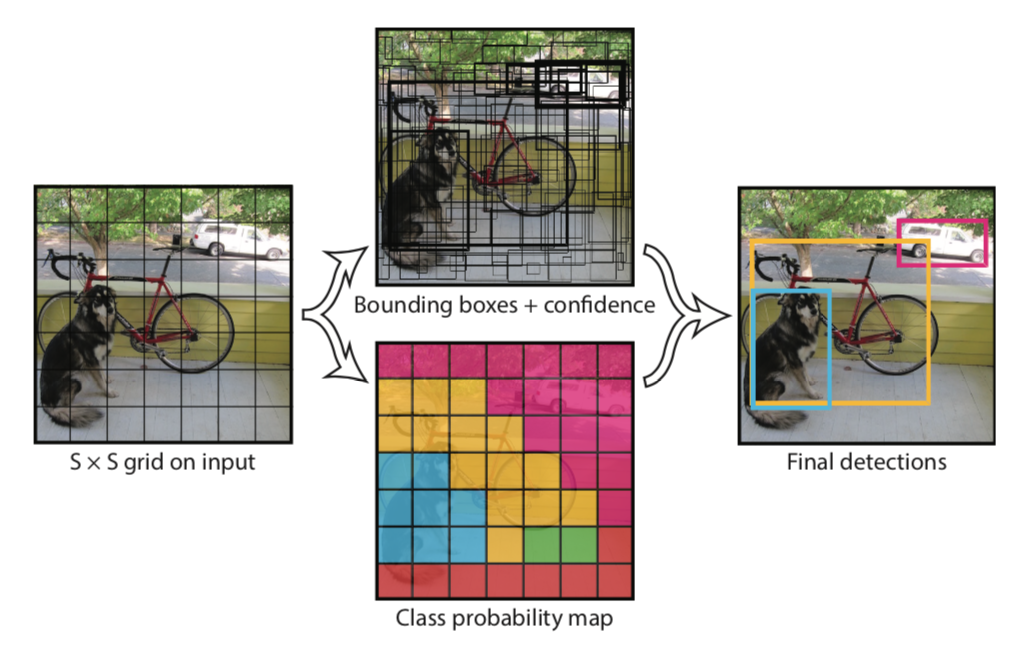
\includegraphics[scale=0.8]{img/yolo_detekcija.png}
	\caption{Prikaz detekcije objekata YOLO modelom.}
	\label{yolo_detekcija}
\end{figure}

\subsection{YOLO v2}
YOLO v2, \cite{DBLP:journals/corr/RedmonF16}, je poboljšana inačica YOLO modela koja omogućava podešavanje ravnoteže između brzine i preciznosti tako da radi s različitim veličinama slike. Ako model na ulazu dobije veće slike, bit će sporiji, ali precizniji i obrnuto tome, ako na ulazu dobije manje slike, bit će brži ali manje precizan. Ako obrađuje 40 slika u sekundi, na skupu podataka Pascal VOC 2007 (\cite{pascal-voc-2007}) postiže bolje rezultate od Faster R-CNN-a i SSD-a i znatno je brži. YOLO v2 za razliku od originalnog YOLO modela ne predviđa prozore direktno nego koristi "sidra" pa predviđa promijene unaprijed određenog prozora kao što radi i Faster R-CNN. Za razliku od Faster R-CNN-a kod kojeg se "sidra" biraju ručno, YOLO v2 ih određuje provođenjem algoritma K srednjih vrijednosti nad prozorima u skupu podataka za trening. Udaljenost prozora od centroida računa se formulom $d(prozor, centroid) = 1 - IOU(prozor, centroid)$, gdje je $IOU$ omjer presjeka i unije prozora i centroida.
Da bi model mogao raditi s različitim veličinama slika, tijekom treninga se mijenjaju veličine ulaznih slika kako bi mreža naučila detektirati objekte neovisno o veličini slike.  
Zbog dodatnog ubrzanja modela, YOLO v2 koristi manju konvolucijsku mrežu, Darknet-19, čija je arhitektura temeljena na Googlenet arhitekturi. 
Autori također treniraju model YOLO9000 koji koristi YOLO v2 arhitekturu, ali se paralelno trenira za klasifikaciju i detekciju te može detektirati 9000 različitih razreda objekata.

\subsection{YOLO v3}
YOLO v3, \cite{DBLP:journals/corr/abs-1804-02767}, uvodi nekoliko manjih promjena u odnosu na YOLO v2 koje povećavaju preciznost modela.
Predviđanje prozora se radi u odnosu na centroide dobivene provođenjem algoritma K srednjih vrijednosti kao i kod YOLO v2. Za klasifikaciju se ne koristi softmax da bi se omogućila pripadnost objekta u više razreda, kao kod YOLO9000.
Novost u odnosu na prethodni model je da radi predikciju na 3 skale. Detekcija se radi tako da se na 3 mape značajki na različitim mjestima u mreži primjene jezgre dimenzija $1 \times 1$. Ukupna veličina jezgre je $1 \times 1 \times (B \times (5 + C))$, gdje je $B$ broj predviđenih prozora, a C broj razreda. Još jedna novost je nova arhitektura konvolucijske mreže, Darknet-53. Darknet-53 se sastoji od 53 konvolucijska sloja što je veće od mreže korištene u YOLO v2 pa je detekcija sporija, ali povećava preciznost modela. 
U usporedbi s YOLO v2, YOLO v3 je bolji u detekciji malih objekata, ali je lošiji u detekciji srednjih i velikih objekata.

 